\documentclass[a4paper]{article}
\usepackage{geometry}
%\usepackage[nostamp,tikz,svg]{moodle}
\usepackage[handout,nostamp,tikz,svg]{moodle}
\pagestyle{empty}
 \geometry{
 a4paper,
 total={175mm,260mm},
 left=15mm,
 top=15mm,
 }

\usepackage{fontspec}
\usepackage{graphicx}
\usepackage{hyperref,babel}
\usepackage[cm]{fullpage}
\usepackage{fancyvrb}

\pagestyle{empty}

\begin{document}

\begin{quiz}{SelectionES1\_EN}

\begin{matching}[points=1,shuffle]{3.2-01. UDP multiplexing and demultiplexing.}
\textbf{3.2-01. UDP multiplexing and demultiplexing.} 

Consider the figure below, with 6 sockets shown across the network, and the corresponding Python code at each host. There are four UDP segments in flight. Match the source and destination port numbers for each segment with a value below. 

\begin{center}
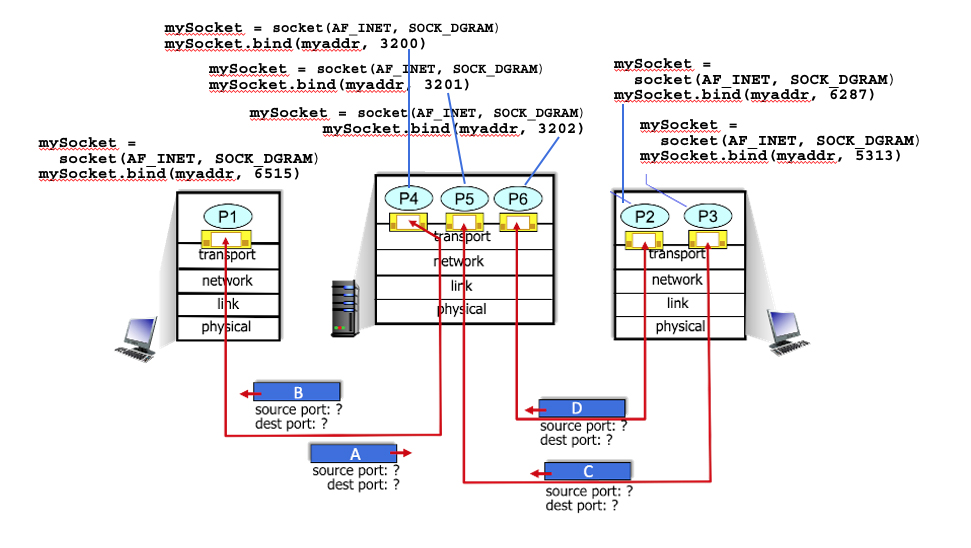
\includegraphics[width=\linewidth]{figs/fig1.jpg}
\end{center}
\item Segment A source port \# \answer 6515
\item Segment B source port \# \answer 3200
\item Segment C source port \# \answer 5313
\item Segment C destination port \# \answer 3201
\item Segment D source port \# \answer 6287
\item Segment D destination port \# \answer 3202
\end{matching}

\begin{multi}[points=1]{2.2-09. HTTP/2 versus HTTP/1.1: object download delays.}
\textbf{2.2-09. HTTP/2 versus HTTP/1.1: object download delays.} 

Consider a client and a server, separated by an RTT of 4 time units. The client makes a request for 4 objects at t=0. O1 consists of 10 frames, O2 and O4 each consist of 1 frame, and O3 consists of 2 frames.  In the HTTP/2 example shown in the figure, the server is transmitting frames to the client in the order O1, O2, O3, O4 (as long as there are frames of type i to transmit, and when not the server just moves on to a frame from object i+1 mod 4).  Each frame takes 1 time unit to transmit. 

\begin{center}
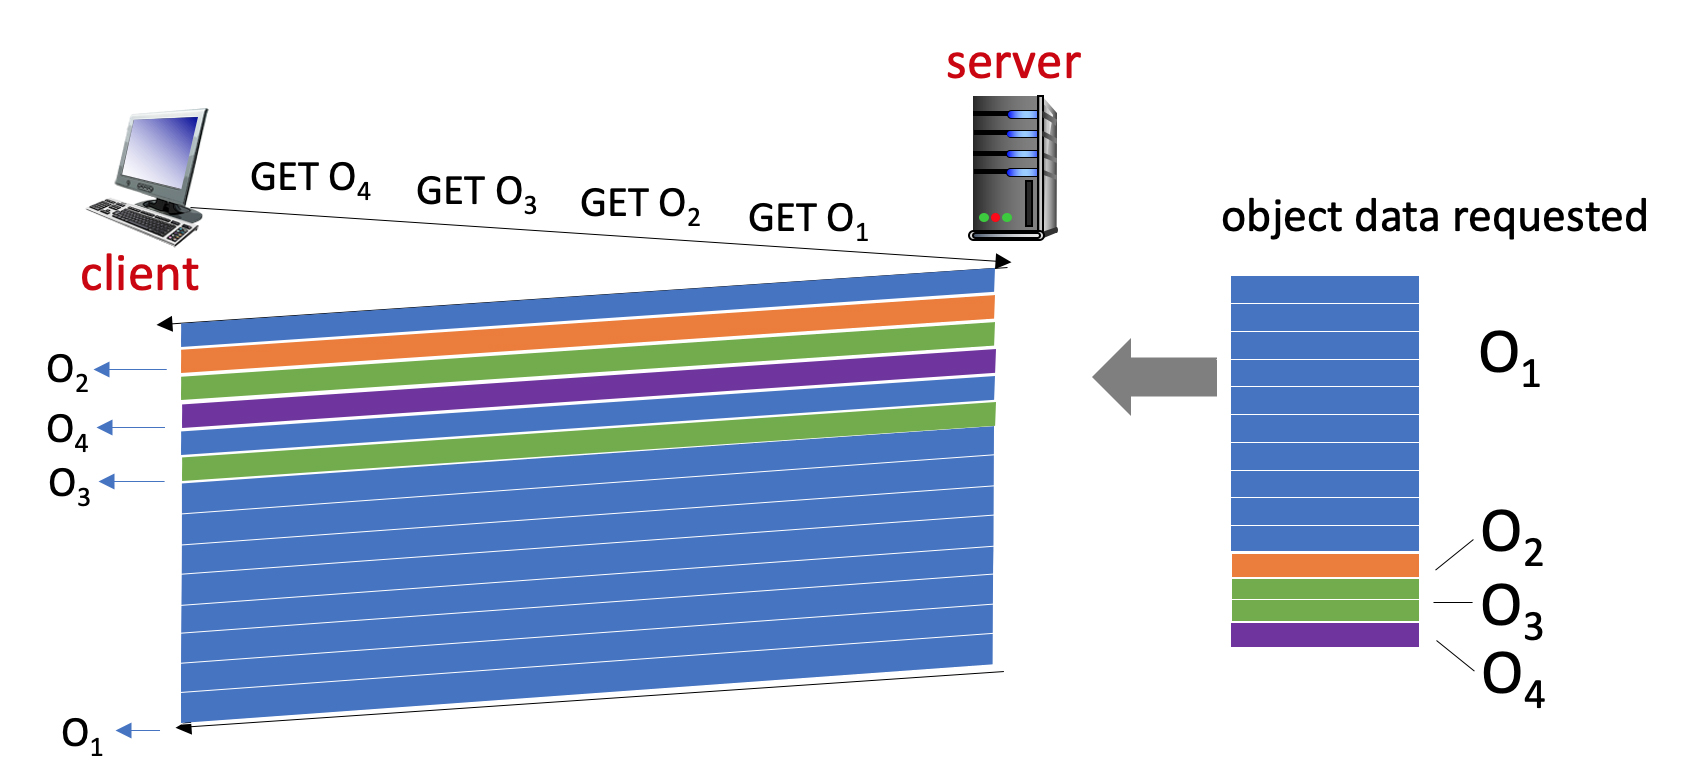
\includegraphics[width=\linewidth]{figs/2.2.9.jpg}
\end{center}

Under HTTP 1.1, the server would send O1, O2, O3, O4 in that first-come-first-served (FCFS) order, sending each object in its entirety before moving on to send the next object in that order. Let's define the object download delay as the time from when an object is requested (at t=0 below) to the time that object is received in its entirety. What is the average object download delay (the sum of the four object download delays divided by 4) under the HTTP/2 object frame transmission order shown in the figure and under HTTP/1.1 O1, O2, O3, O4 object transmission order?
\item* Average object download delay under HTTP/1.1: 16.0, under HTTP/2: 10.5
\item Average object download delay under HTTP/1.1: 14.0, under HTTP/2: 9.5
\item Average object download delay under HTTP/1.1: 18.0, under HTTP/2: 14.0
\item Average object download delay under HTTP/1.1: 12.5, under HTTP/2: 10.0
\item Average object download delay under HTTP/1.1: 24.0, under HTTP/2: 18.0
\item Average object download delay under HTTP/1.1: 22.0, under HTTP/2: 17.5
\end{multi}

\begin{multi}[points=1,shuffle]{2.4-02. DNS: time to resolve query.}
\textbf{2.4-02. DNS: time to resolve query.}  

Suppose that the local DNS server caches all information coming in from all root, TLD, and authoritative DNS servers for 20 time units. (Thus, for example, when a root server returns the name and address of a TLD server for .com, the cache remembers that this is the TLD server to use to resolve a .com name).  

Assume also that the local cache is initially empty, that iterative DNS queries are always used, that DNS requests are just for name-to-IP-address translation, that 1 time unit is needed for each server-to-server or host-to-server (one way) request or response, and that there is only one authoritative name server (each) for any .edu or .com domain. 
\begin{center}
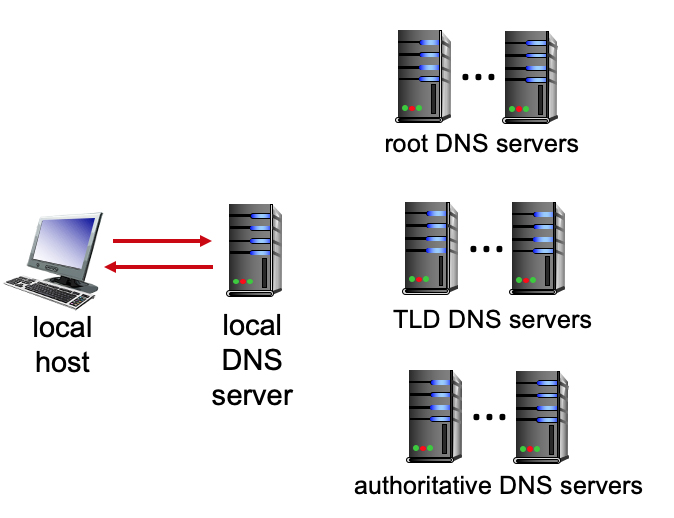
\includegraphics[width=\linewidth]{figs/2.4.4.jpg}
\end{center}

Consider the following DNS requests, made by the local host at the given times:
\begin{itemize}
	\item t=0, the local host requests that the name gaia.cs.umass.edu be resolved to an IP address. 
	\item t=1, the local host requests that the name web.cs.umass.edu be resolved to an IP address
\end{itemize}

How many time units are needed for the DNS request made at \textbf{t=1} to be resolved?
\item 2 time units.
\item 4 time units.
\item 6 time units.
\item 8 time units.
\item* 10 time units.
\end{multi}

\begin{multi}[points=1,shuffle]{2.6-2. Playout delay: minimum playout delay.}
\textbf{2.6-2. Playout delay: minimum playout delay.}

Consider the following scenario, in which a server is streaming chunks of video to a client. The first chunk is transmitted by the server at \textbf{t=2}, is received at the client at \textbf{t=10}, and is playout out at the client at \textbf{t=16}.  The retransmission, reception, and playout of 11 chunks is shown. 

In this example, the playout delay is 6, and no chunks miss their playout deadline.
\begin{center}
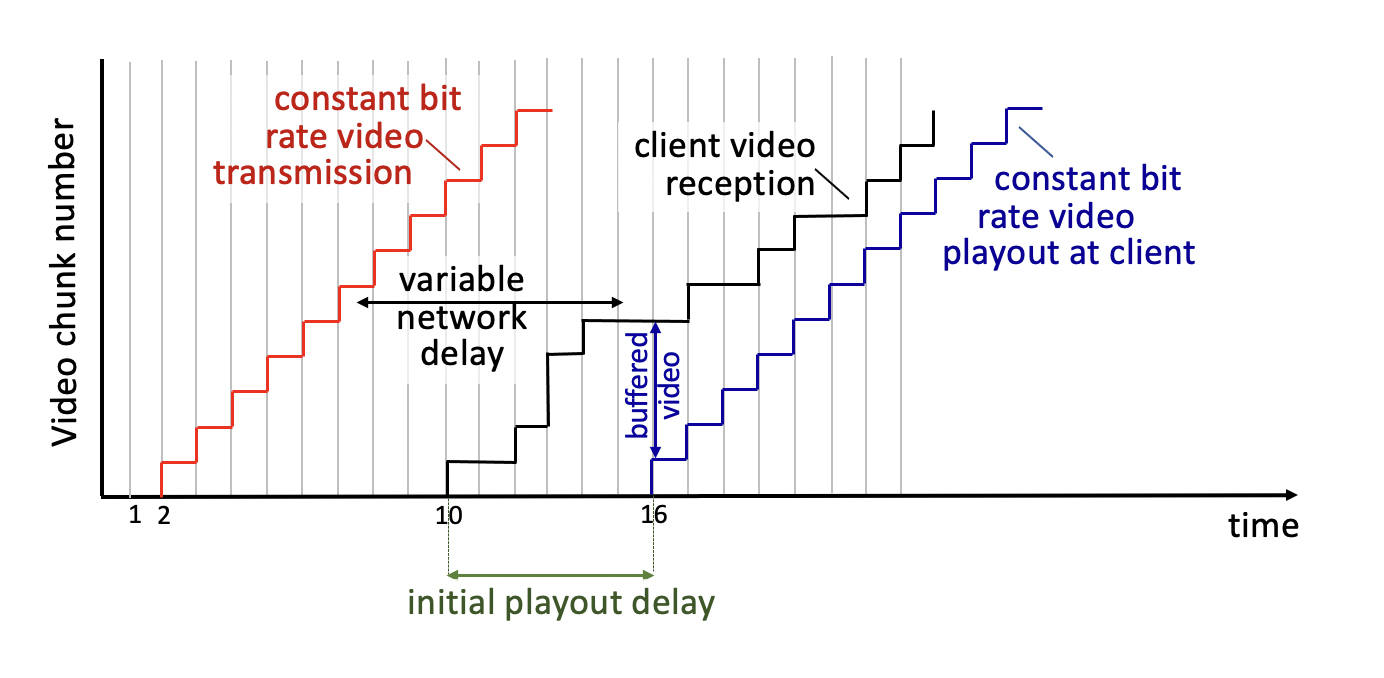
\includegraphics[width=\linewidth]{figs/playout_delay.jpg}
\end{center}

What is the \textbf{smallest} initial playout delay such that the (periodic) playout of chunks is timed such that no chunks miss their playout deadline? You can assume that if a chunk arrives (black staircase) at the same time as it is scheduled for playout (blue staircase), then the chunk is played out successfully without being lost.
\item 1
\item 2
\item 3
\item* 4
\item 5
\item 6
\item It isn't possible.
\end{multi}

\begin{multi}[points=1,shuffle]{3.5-2a. TCP sequence and ACK numbers.}
\textbf{3.5-2a. TCP sequence and ACK numbers.}

Consider the figure below, where a TCP sender sends 8 TCP segments at \emph{t = 1, 2, 3, 4, 5, 6, 7, 8.} Suppose the initial value of the sequence number is 0 and every segment sent to the receiver contains 100 bytes. The delay between the sender and receiver is 5 time units, and so the first segment arrives at the receiver at t = 6. The ACKs sent by the receiver at \emph{t = 6, 7, 8, 10, 11, 12} are shown. The TCP segments (if any) sent by the sender at \emph{t = 11, 13, 15, 16, 17, 18} are \emph{not} shown. The segment sent at \emph{t=4} is lost, as is the ACK segment sent at \emph{t=7}. 
\begin{center}
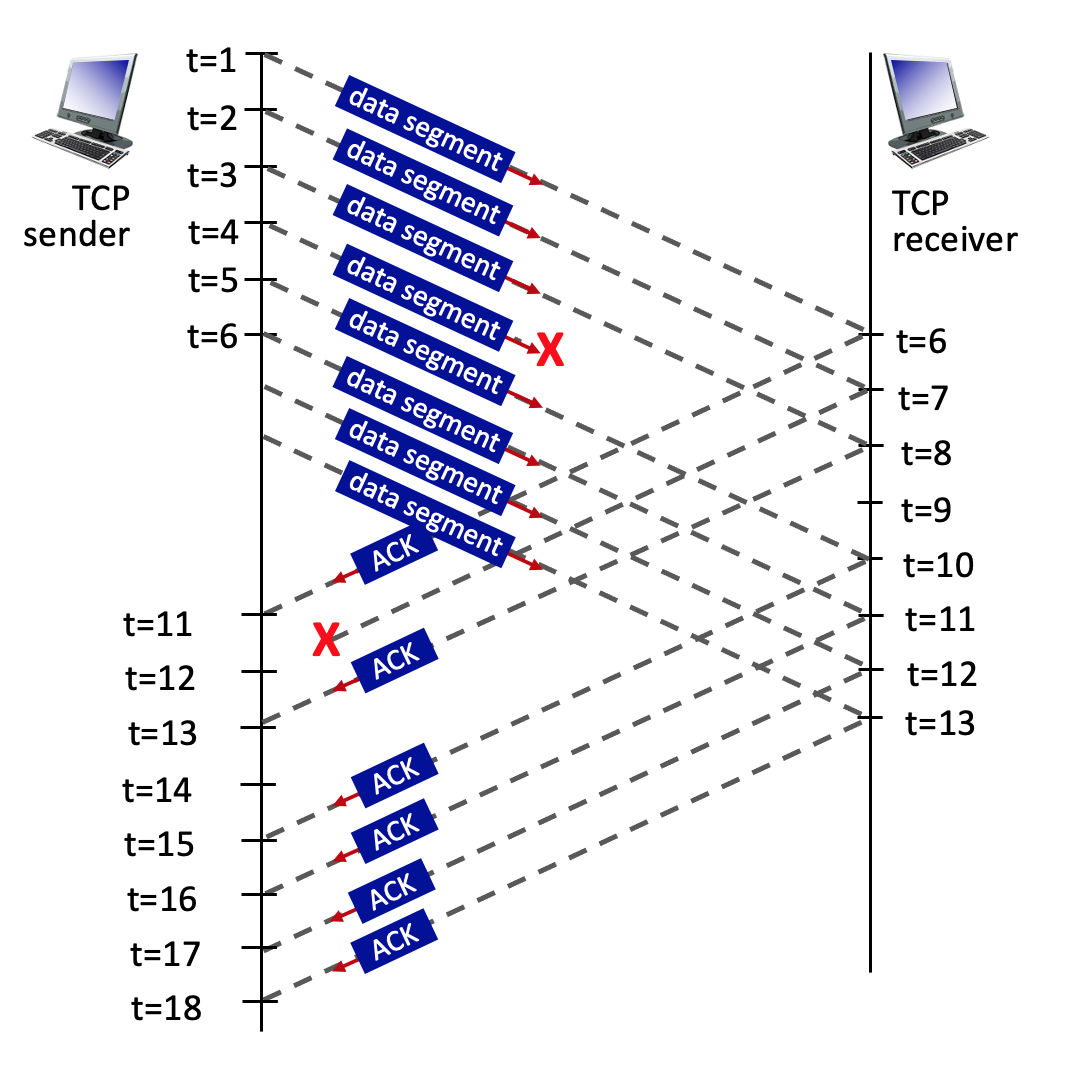
\includegraphics[width=\linewidth]{figs/tcp_seq_ack_1.jpg}
\end{center}

 What is the sequence number of the segment sent at \emph{t=2}?
\item 200
\item* 100
\item 1
\item 2
\end{multi}

\begin{multi}[points=1,shuffle]{3.5-2b. TCP sequence and ACK numbers (b).}
\textbf{3.5-2b. TCP sequence and ACK numbers (b). }

Consider again the figure below (as in question 3.5-2a) where a TCP sender sends 8 TCP segments at \emph{t = 1, 2, 3, 4, 5, 6, 7, 8} and the segment sent at \emph{t=4} is lost, as is the ACK segment sent at \emph{t=7}. What is the ACK value carried in the receiver-to-sender ACK sent at \emph{t=6}?
\begin{center}
	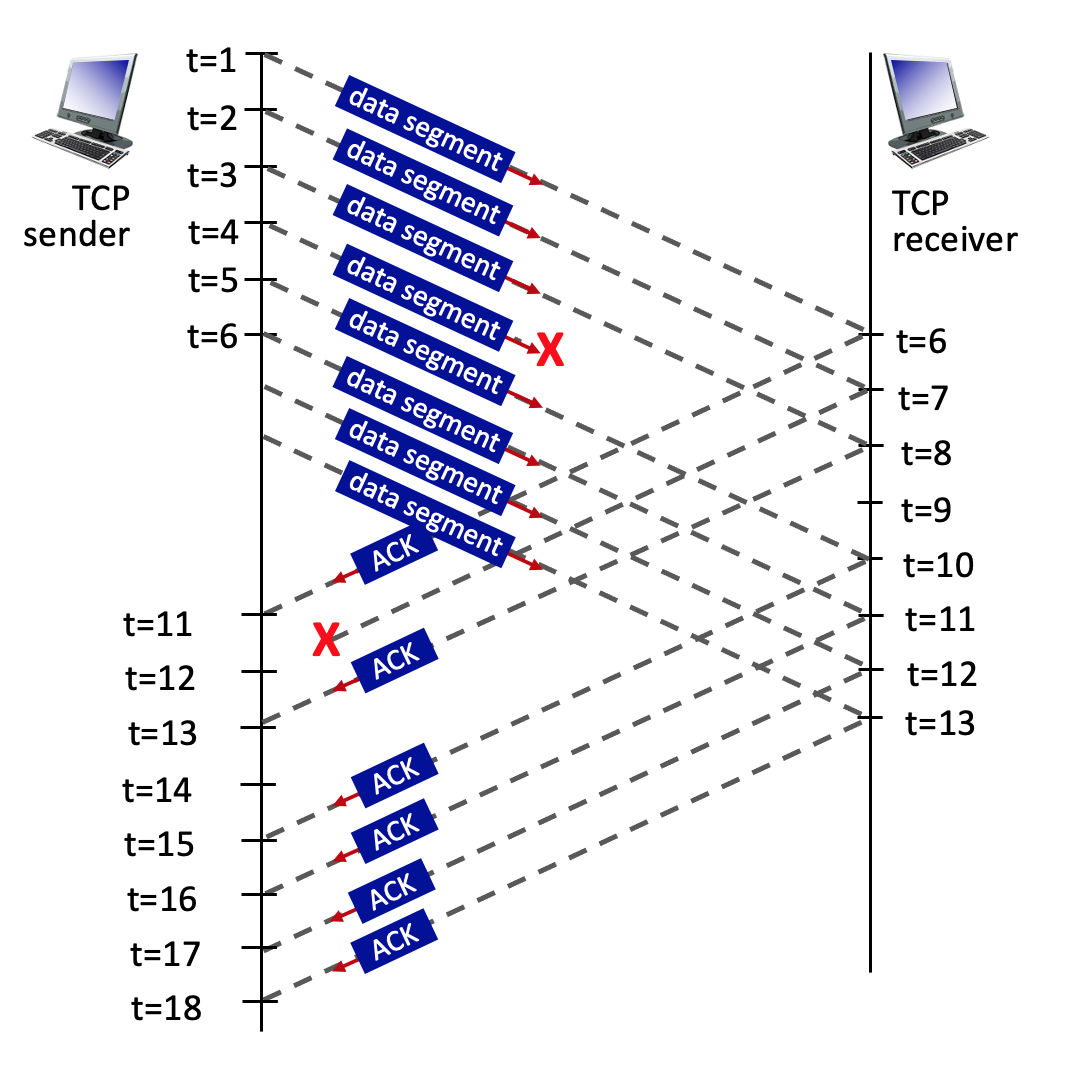
\includegraphics[width=\linewidth]{figs/tcp_seq_ack_1.jpg}
\end{center}
\item 200
\item* 100
\item 1
\item 2
\item 0
\item None of these other answers.
\end{multi}

\begin{multi}[points=1,shuffle]{3.5-2c. TCP sequence and ACK numbers (c).}
\textbf{3.5-2c. TCP sequence and ACK numbers (c).}

Consider again the figure below (as in question 3.5-2a) where a TCP sender sends 8 TCP segments at \emph{t = 1, 2, 3, 4, 5, 6, 7, 8} and the segment sent at \emph{t=4} is lost, as is the ACK segment sent at \emph{t=7}. What is the ACK value carried in the receiver-to-sender ACK sent at \emph{t=8}?
\begin{center}
	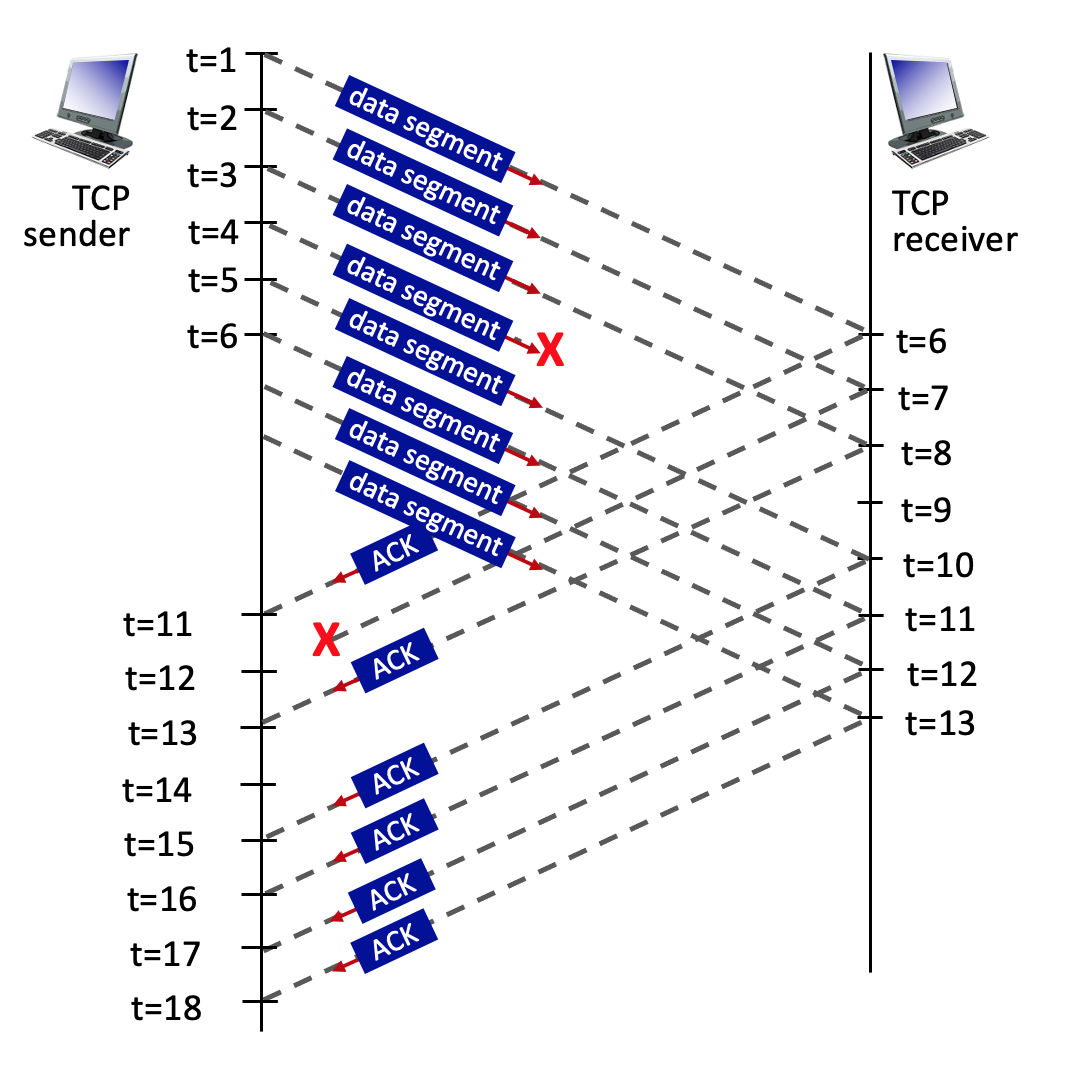
\includegraphics[width=\linewidth]{figs/tcp_seq_ack_1.jpg}
\end{center}
\item 200
\item 100
\item* 300
\item 400
\item 3
\item None of these other answers.
\end{multi}

\begin{multi}[points=1,shuffle]{3.5-2d. TCP sequence and ACK numbers (d).}
\textbf{3.5-2d. TCP sequence and ACK numbers (d).}

Consider again the figure below (as in question 3.5-2a) where a TCP sender sends 8 TCP segments at \emph{t = 1, 2, 3, 4, 5, 6, 7, 8} and the segment sent at \emph{t=4} is lost, as is the ACK segment sent at \emph{t=7}. What is the ACK value carried in the receiver-to-sender ACK sent at \emph{t=10}?
\begin{center}
	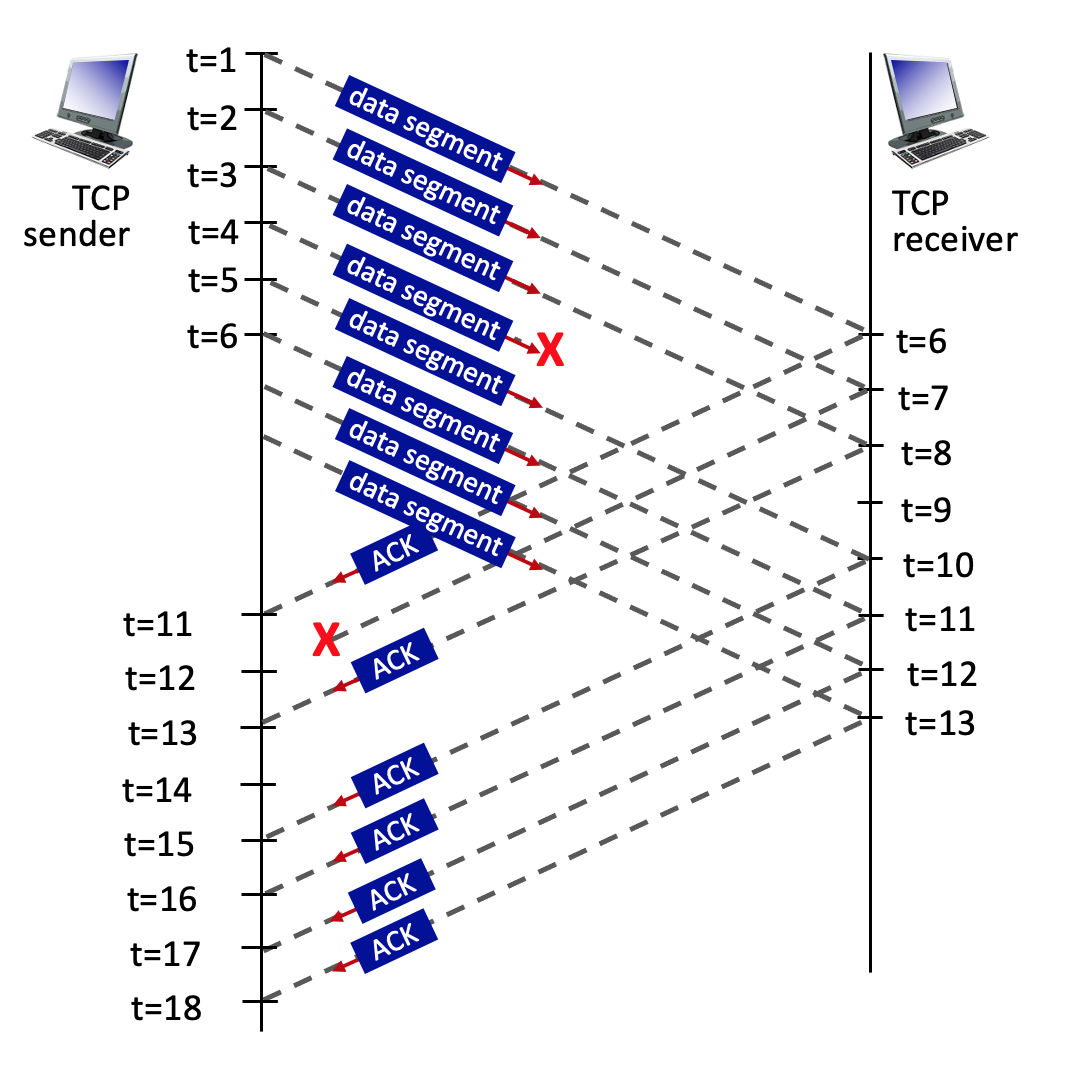
\includegraphics[width=\linewidth]{figs/tcp_seq_ack_1.jpg}
\end{center}
\item 200
\item 100
\item* 300
\item 400
\item 3
\item None of these other answers.
\end{multi}

\begin{multi}[points=1,shuffle]{3.7-1a. TCP congestion control example (a).}
\textbf{3.7-1a. TCP congestion control example (a).}

Consider the figure below, where a TCP sender sends 8 TCP segments at \emph{t = 1, 2, 3, 4, 5, 6, 7, 8.} Suppose the initial value of the sequence number is 0 and every segment sent to the receiver each contains 100 bytes. The delay between the sender and receiver is 5 time units, and so the first segment arrives at the receiver at \textbf{t=6}. The ACKs sent by the receiver at \emph{t = 6, 7, 8, 10, 11, 12} are shown. The TCP segments (if any) sent by the sender at \textbf{t = 11, 13, 15, 16, 17, 18} are \emph{not} shown. The segment sent at \textbf{t=4} is lost, as is the ACK segment sent at \textbf{t=7}. 

\begin{center}
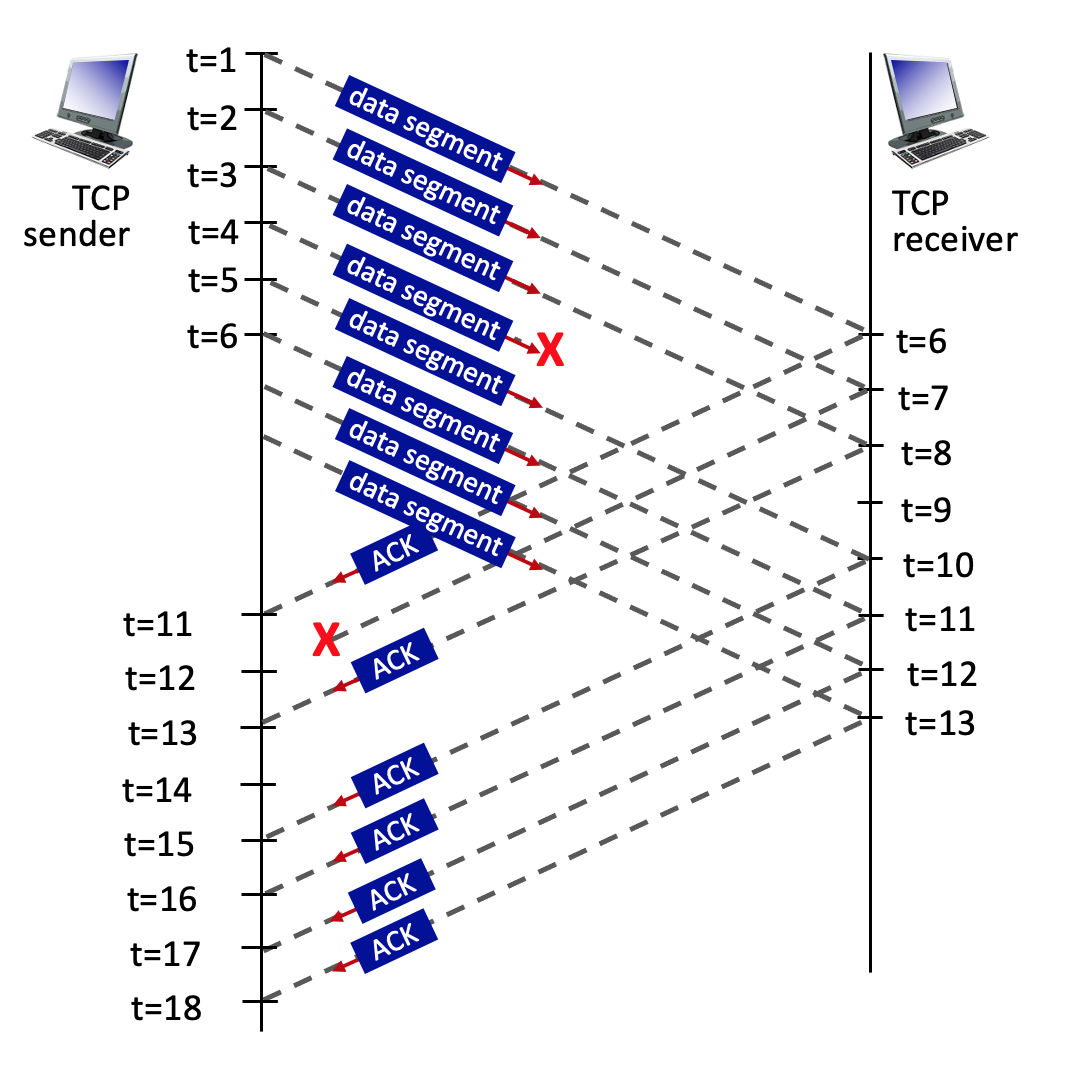
\includegraphics[width=\linewidth]{figs/tcp_seq_ack_1.jpg}
\end{center}

What is the sender action at \textbf{t = 11} upon receipt of the ACK?
\item Increase the congestion window size, move the window base forward by 2, and send new segments, as available and as allowed by the congestion window.
\item* Increase the congestion window size, move the window base forward by 1, and send new segments, as available and as allowed by the congestion window.
\item Keep the congestion window size the same but send new segments, as available and as allowed by the congestion window.
\item Do nothing.
\item Send an ACK to the ACK.
\end{multi}

\begin{multi}[points=1,shuffle]{3.7-1b. TCP congestion control example (b).}
\textbf{3.7-1b. TCP congestion control example (b).}

Consider again the figure below (as in question 3.7-1a), where a TCP sender sends 8 TCP segments at \emph{t = 1, 2, 3, 4, 5, 6, 7, 8} and the segment sent at \textbf{t=4} is lost, as is the ACK segment sent at \textbf{t=7}. 

\begin{center}
	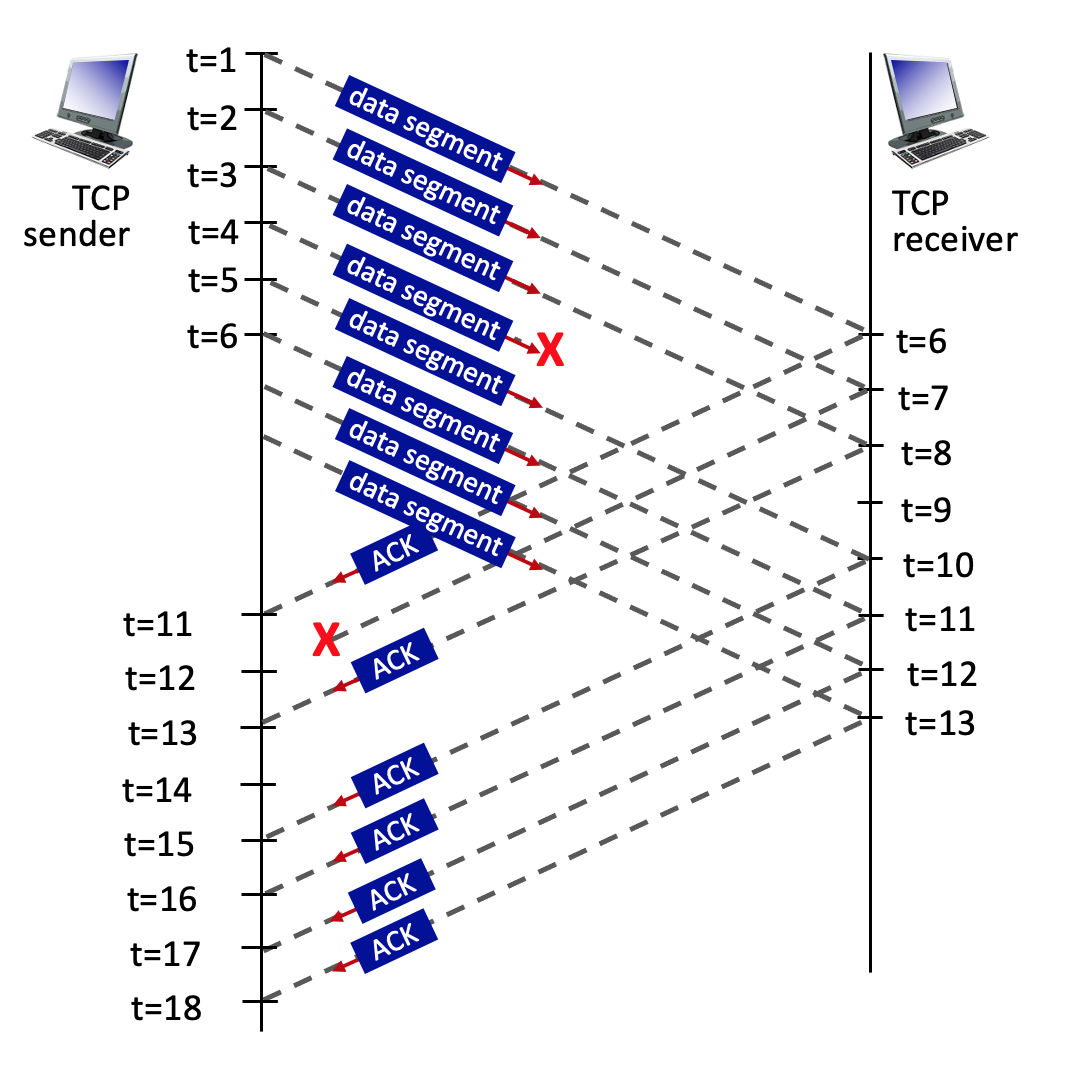
\includegraphics[width=\linewidth]{figs/tcp_seq_ack_1.jpg}
\end{center}

What is the sender action at \textbf{t=13} upon receipt of the ACK?
\item* Increase the congestion window size, move the window base forward by 2, and send new segments, as available and as allowed by the congestion window.
\item Increase the congestion window size, move the window base forward by 1, and send new segments, as available and as allowed by the congestion window.
\item Keep the congestion window size the same. Increment the duplicate ACK count by 1.
\item Do nothing.
\item Send an ACK to the ACK.
\end{multi}

\begin{multi}[points=1,shuffle]{3.7-1c. TCP congestion control example (c).}
\textbf{3.7-1c. TCP congestion control example (c).}

Consider again the figure below (as in question 3.7-1a), where a TCP sender sends 8 TCP segments at \emph{t = 1, 2, 3, 4, 5, 6, 7, 8} and the segment sent at \textbf{t=4} is lost, as is the ACK segment sent at \textbf{t=7}. 

\begin{center}
	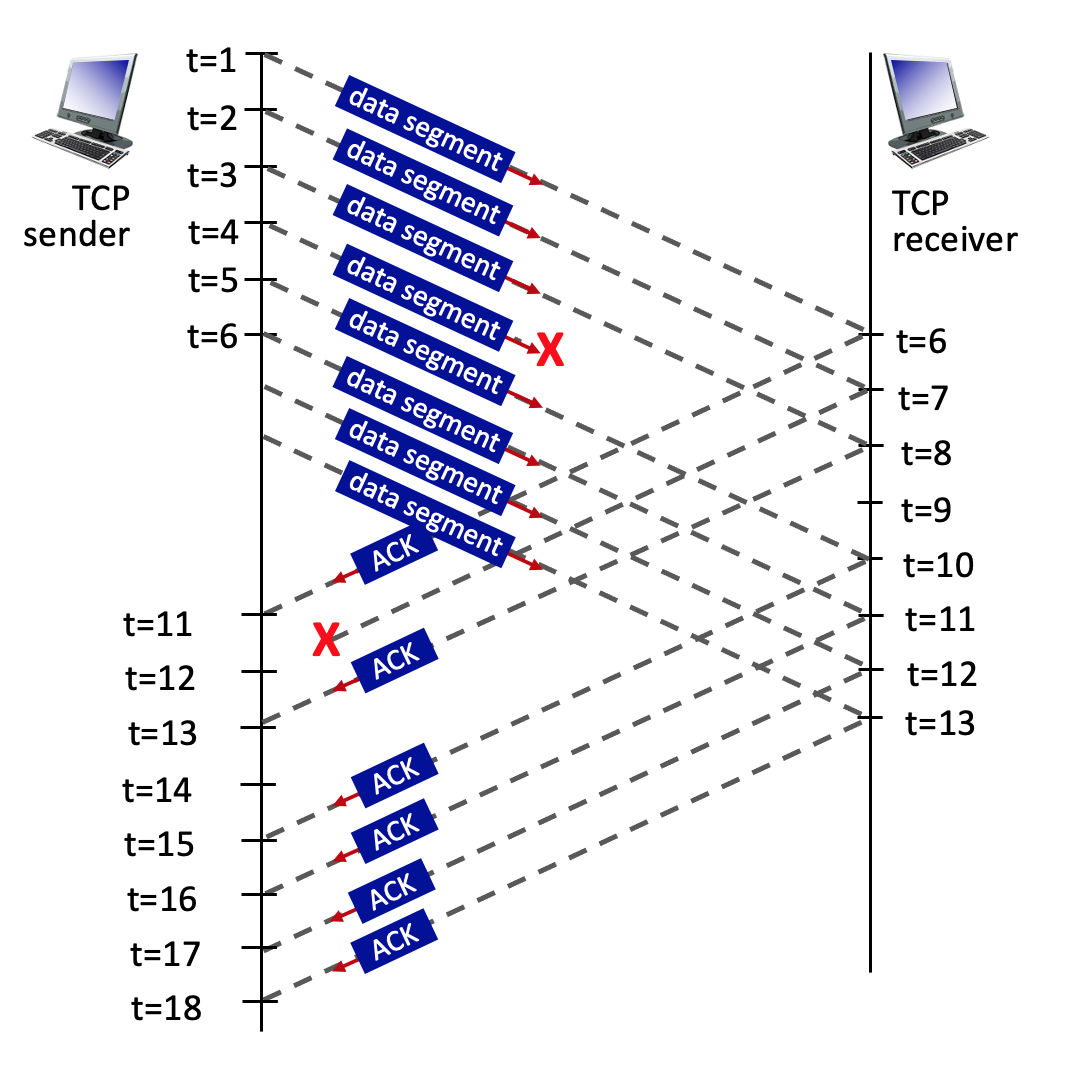
\includegraphics[width=\linewidth]{figs/tcp_seq_ack_1.jpg}
\end{center}

What does the sender do at \textbf{t=16}? You can assume for this question that no timeouts have occurred.
\item Sets its cwnd window value to 1, and retransmit the segment with sequence number 300.
\item Cut its value of cwnd in half, and retransmit the segment with sequence number 300.
\item Inform the upper layer that the connection is terminated, and close the socket.
\item* Do nothing except increment the number of duplicate ACKs received by 1.
\end{multi}

\begin{multi}[points=1,shuffle]{3.7-1d. TCP congestion control example (d).}
\textbf{3.7-1d TCP congestion control example (d).}

Consider again the figure below (in question 3.7-1a), where a TCP sender sends 8 TCP segments at \emph{t = 1, 2, 3, 4, 5, 6, 7, 8} and the segment sent at \textbf{t=4} is lost, as is the ACK segment sent at \textbf{t=7}. 

\begin{center}
	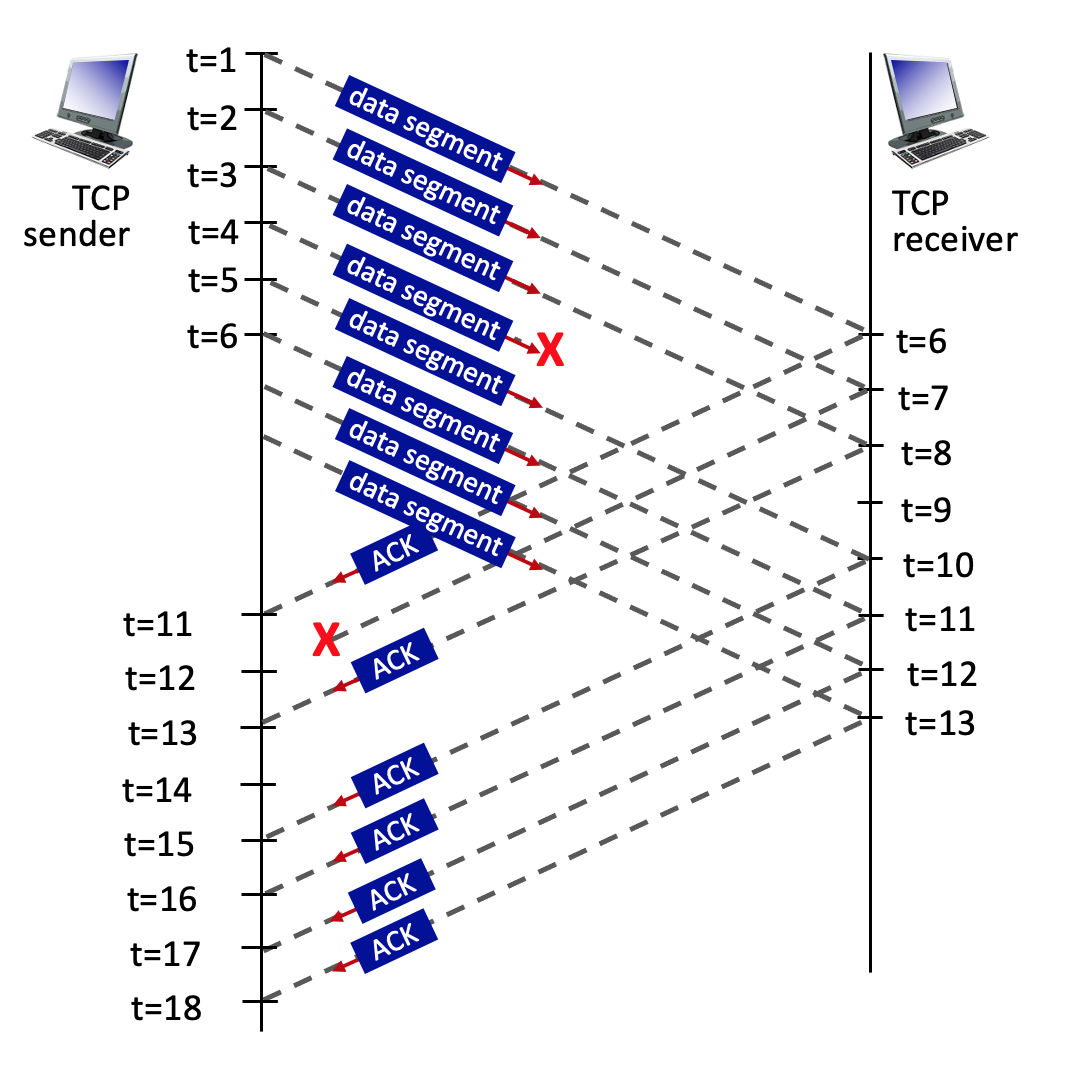
\includegraphics[width=\linewidth]{figs/tcp_seq_ack_1.jpg}
\end{center}

What does the sender do at \textbf{t=17}? You can assume for this question that no timeouts have occurred.
\item Sets its cwnd window value to 1, and retransmit the segment with sequence number 300.
\item* Cut its value of cwnd in half, and retransmit the segment with sequence number 300.
\item Inform the upper layer that the connection is terminated, and close the socket.
\item Do nothing except increment the number of duplicate ACKs by 1.
\end{multi}

\begin{multi}[points=1,shuffle]{3.7-1e. TCP congestion control example (e).}
\textbf{3.7-1e. TCP congestion control example (e).}

Consider again the figure below (in question 3.7-1a), where a TCP sender sends 8 TCP segments at \emph{t = 1, 2, 3, 4, 5, 6, 7, 8} and the segment sent at \textbf{t=4} is lost, as is the ACK segment sent at \textbf{t=7}. 

\begin{center}
	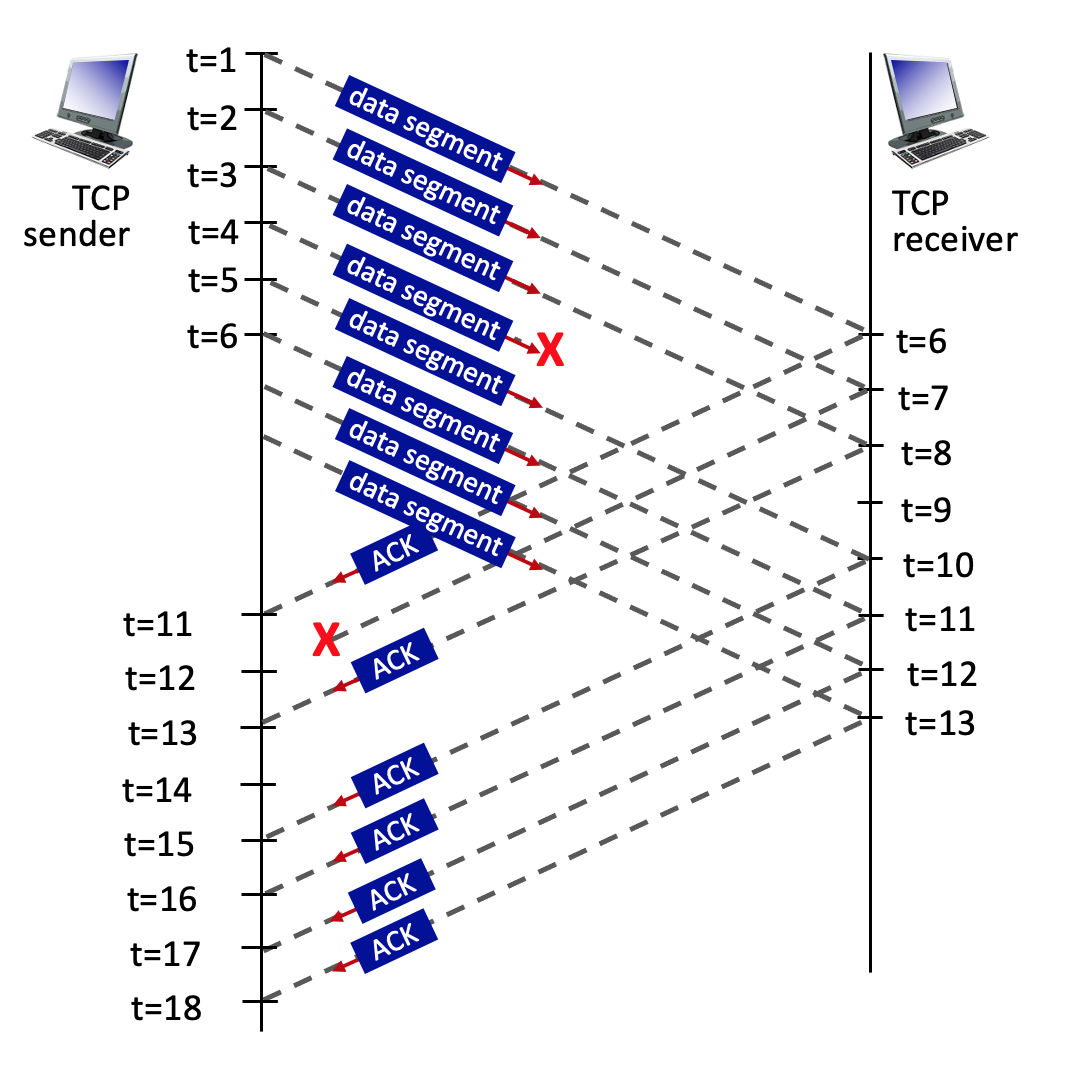
\includegraphics[width=\linewidth]{figs/tcp_seq_ack_1.jpg}
\end{center}

Suppose that the next event after \textbf{t=17} is a timeout event.  What does the sender do?
\item* Sets it its cwnd window value to 1, and retransmit the segment with sequence number 300.
\item Sets it its cwnd window value to 1, a, and retransmit the segment with sequence number 100.
\item Inform the upper layer that the connection is terminated, and close the socket.
\item Do nothing.
\item Cut its cwnd window value in half, and retransmit the segment with sequence number 300.
\end{multi}

\begin{multi}[points=1,shuffle,multiple]{3.7-2a. Phases of TCP congestion control (a).}
\textbf{3.7-2a Phases of TCP congestion control (a).} 

Consider the figure below, which plots the evolution of TCP's congestion window at the beginning of each time unit (where the unit of time is equal to the RTT). In the abstract model for this problem, TCP sends a ``flight'' of packets of size cwnd at the beginning of each time unit. The result of sending that flight of packets is that either (i) all packets are ACKed at the end of the time unit, (ii) there is a timeout for the first packet, or (iii) there is a triple duplicate ACK for the first packet. 

During which of the following intervals of time is TCP performing slow start?
\begin{center}
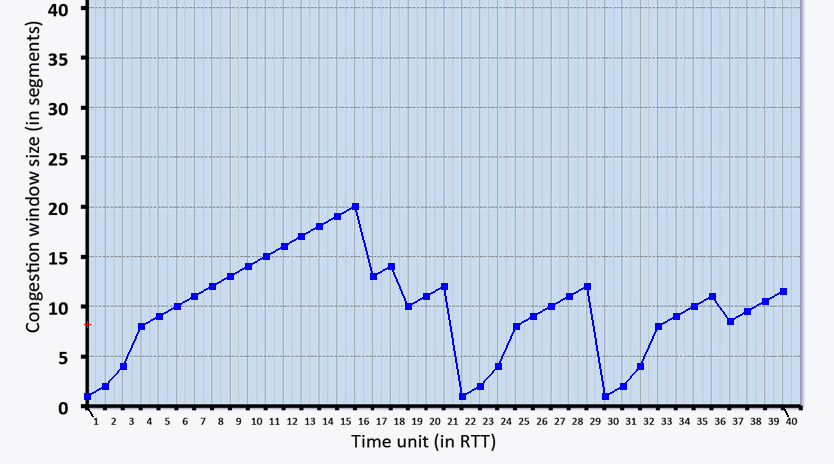
\includegraphics[width=\linewidth]{figs/tcp_cc_evolution.jpg}
\end{center}

\item[fraction=50] $[1,3]$
\item $[4,15]$
\item 16
\item 17
\item 18
\item $[19,20]$
\item 21
\item[fraction=50] $[22,24]$
\end{multi}

\begin{multi}[points=1,shuffle,multiple]{3.7-2b. Phases of TCP congestion control (b).}
\textbf{3.7-2b Phases of TCP congestion control (b).} 

Consider again the figure below (question 3.7-2a) showing the evolution of TCP's congestion window size. In this figure, during which of the following intervals of time is TCP performing congestion avoidance?

\begin{center}
	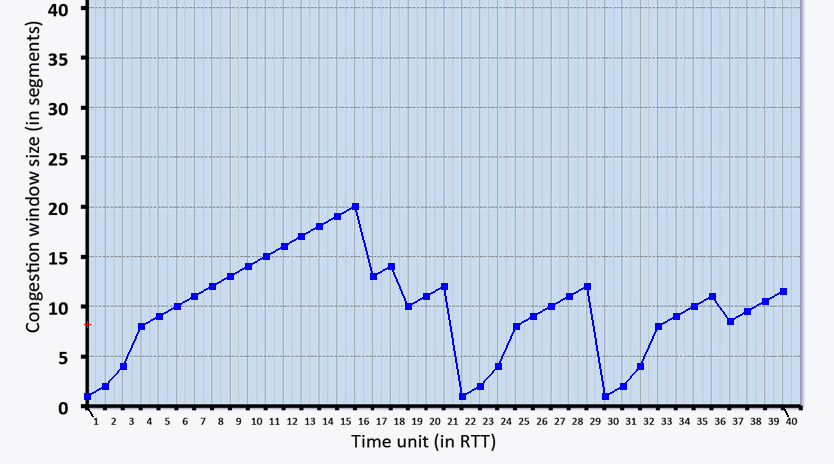
\includegraphics[width=\linewidth]{figs/tcp_cc_evolution.jpg}
\end{center}
\item $[1,3]$
\item[fraction=33.33333] $[4,15]$
\item 16
\item[fraction=33.33333] 17
\item 18
\item[fraction=33.33333] $[19,20]$
\item 21
\item $[22,24]$
\end{multi}

\begin{multi}[points=1,shuffle,multiple]{3.7-2c. Phases of TCP congestion control (c).}
\textbf{3.7-2c Phases of TCP congestion control (c).} 

Consider again the figure below (question 3.7-2a) showing the evolution of TCP's congestion window size. In this figure, at the end of which units of time does TCP detect a triple-duplicate-ACK?

\begin{center}
	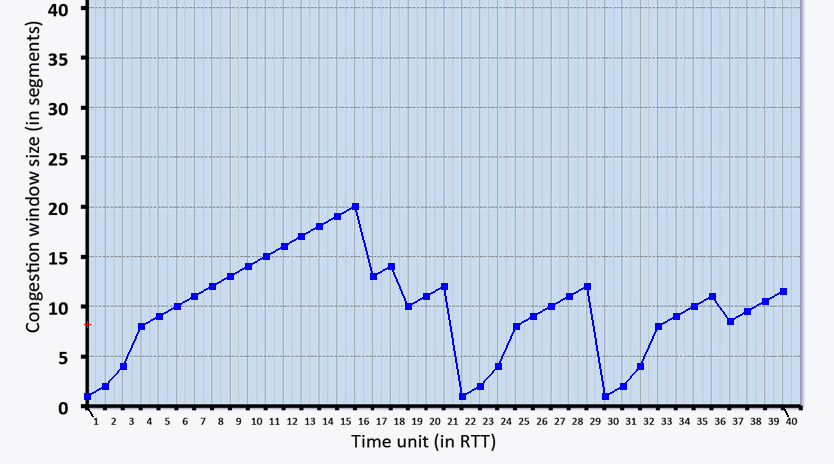
\includegraphics[width=\linewidth]{figs/tcp_cc_evolution.jpg}
\end{center}
\item $[1,3]$
\item $[4,15]$
\item[fraction=50] 16
\item 17
\item[fraction=50] 18
\item $[19,20]$
\item 21
\item $[22,24]$
\end{multi}

\begin{multi}[points=1,shuffle]{3.7-2d. Phases of TCP congestion control (d).}
\textbf{3.7-2d. Phases of TCP congestion control (d).} 

Consider again the figure above (question 3.7-2a) showing the evolution of TCP's congestion window size. In this figure, at the end of which unit(s) of time does TCP detect a loss via timeout? 

\begin{center}
	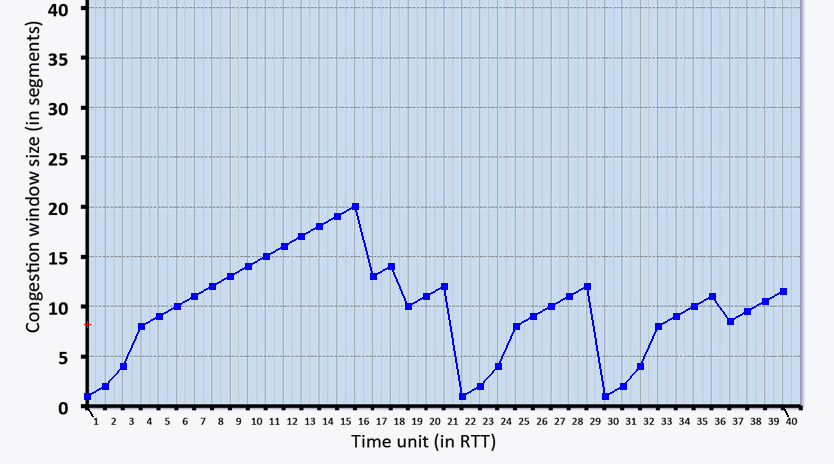
\includegraphics[width=\linewidth]{figs/tcp_cc_evolution.jpg}
\end{center}
\item $[1,3]$
\item $[4,15]$
\item 16
\item 17
\item 18
\item $[19,20]$
\item* 21
\item $[22,24]$
\end{multi}

\begin{shortanswer}[points=1,shuffle]{3.5-1a. TCP RTT estimation and timeout value.}
\textbf{3.5-1a. TCP RTT estimation and timeout value}. 

Suppose that TCP's current estimated values for the round trip time (\textbf{estimatedRTT}) and deviation in the RTT (\textbf{DevRTT}) are 300 msec and 13 msec, respectively. Suppose that the next two measured RTTs are 330 msec and 240 msec respectively. 

We want to calculate TCP's RTT estimate, and the value of TCP's timeout interval. Note that given a new measured RTT, you should first compute \textbf{devRTT}, then \textbf{estimatedRTT}, and then (lastly) the timeout interval. 

Use the values of $\alpha$ = 0.125, $\beta$ = 0.25. Following the newly measured RTT of 330 msec, what is the new value for \textbf{devRTT} in msec? [Note: round your answer to the nearest msec -- enter an integer value, do not include any decimal places/point or any leading zeros]
\item* 17
\end{shortanswer}

\end{quiz}
\end{document}
